\documentclass[010-intro.tex]{subfiles}

\begin{document}

\subsection{Where the Term ``Data Science'' Originated}

    In 1962, John Tukey describes data analysis as ``intrinsically an empirical science'',
    and points to electronic computers as being vital to data analysis
    \cite{tukeyFutureDataAnalysis1962, pressVeryShortHistory2013}.
    This scientific approach to data analysis,
    with hypothesis driven exploration,
    was later called ``Exploratory Data Analysis'' (EDA).
    In 1977,
    Tukey calls for exploratory data analysis to be used along with confirmatory data analysis
    by understanding the data first before calculating any confirmatory statistic
    \cite{tukeyExploratoryDataAnalysis1977}.
    
    EDA becomes a core component of what later becomes ``data science'',
    which Peter Naur defines in 1974 as \cite{pressVeryShortHistory2013}:
    \begin{displayquote}
        The science of dealing with data,
        once they have been established,
        while the relation of the data to what they represent
        is delegated to other fields and sciences.
    \end{displayquote}
    While data science as a term or field did not take on mainstream adoption as
    a specific term for the type of skills needed to work with data,
    statisticians realized that many of the kinds of insights they gather
    come from using computational tools
    \cite{tukey1965technical, bradstreet1996teaching}.
    In 1997, C. F. Jeff Wu at the University of Michigan called for a rebranding of
    ``statistics'' and ``statisticians'' in favor of
    ``data science'' and ``data scientists'', respectively,
    since many other ``good'' names were already taken
    (e.g., computer science, information science, material science, cognitive science)
    \cite{pressVeryShortHistory2013}.

    The reliance on computers for statistical computing eventually led to
    John Chambers being awarded the ACM Software System Award in 1998,
    for creating the S system for graphics and data analysis
    (Section \ref{ss:intro-r-history})
    \cite{associationforcomputingmachineryACMSoftwareSystem1998}.
    By 2001, the field of ``data science'' was born with
    William Cleveland's plan at Bell Labs to expand the technical areas of statistics.
    Cleveland proposed six (6) technical areas of data science
    and how university resources should be allocated
    to expand educational and research offerings into the following fields or categories
    \cite{clevelandDataScienceAction2001}:

    \begin{enumerate}
        \item Multidisciplinary Investigations (25\%):
            data analysis collaborations in a collection of subject matter areas
        \item Models and Methods for Data (20\%):
            statistical models;
            methods of model building;
            methods of estimation and distribution based on probabilistic inference.
        \item Computing with Data (15\%):
            hardware systems;
            software systems;
            computational algorithms
        \item Pedagogy (15\%):
            curriculum planning and approaches to teaching for
            elementary school, secondary school, college, graduate school,
            continuing education, and corporate training
        \item Tool Evaluation (5\%):
            surveys of tools in use in practice,
            surveys of perceived needs for new tools,
            and studies of the processes for developing new tools
        \item Theory (20\%):
            foundations of data science;
            general approaches to models and methods, computing with data, teaching, and tool evaluation;
            mathematical investigations of models and methods, computing with data, teaching, and evaluation
    \end{enumerate}

    Universities, along with, government research labs, and corporate research organizations
    have been traditional institutions for innovation.
    These resource allocations shape what is taught to new graduates to progress data science
    \cite{clevelandDataScienceAction2001}.

    Academics typically use journal articles as a means to share knowledge.
    The push to have more Open Access journals, means research and knowledge no longer needs to be put
    behind a paywall.
    In 2002 the ``Data Science Journal'' was launched,
    and by 2003, the ``Journal of Data Science'' was launched.
    Both journals are open access and publish papers on data science education in addition to academic research.
    \cite{DataScienceJournal, JournalDataScience}.

    Hal Varian, Google's Chief Economist, mentions in McKinsey Quarterly in 2009,
    computer engineers was the ``sexy'' job in the 1990s,
    statisticians would be the ``sexy'' job in the next 10 years
    \cite{HalVarianHow2009}.
    Varian alludes to
    the need to visualize and learn from the ubiquitous amount of data and
    many of these skills will need to be transferred to managers who need to understand the data themselves.
    The ``free and ubiquitous'' data and the need to communicate findings will go beyond the professional level,
    and will cascade down to all level of education
    \cite{HalVarianHow2009}.
    As data science becomes a more common term,
    in 2010, Hilary Mason and Chris Wiggins write ``A Taxonomy of Data Science''
    \cite{masonTaxonomyDataScience2010}
    and
    Drew Conway creates ``The Data Science Venn Diagram'' (Figure \ref{fig:conway-venn})
    that aims to clarify what is data science and what skills are needed to be a competent data scientist
    \cite{conwayDataScienceVenn2010}.
    \begin{figure}[!hbtp]
        \centering
        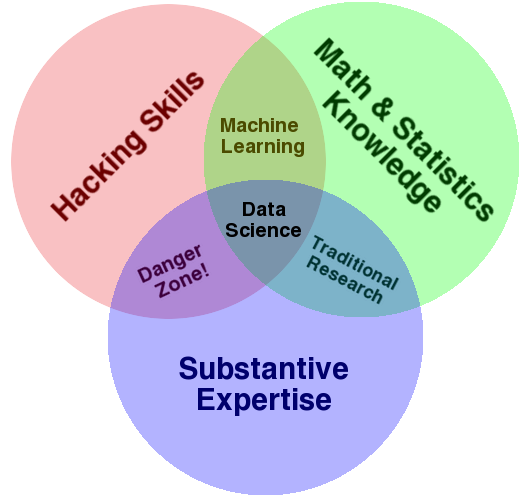
\includegraphics[scale=0.5]{figs/050-intro/Data_Science_VD}
        \caption[Drew Conway's Data Science Venn Diagram]{
        Reproduction of Drew Conway's Data Science Venn Diagram \cite{conwayDataScienceVenn2010}.
        }
        \label{fig:conway-venn}
    \end{figure}
    Mason and Wiggins's ``Snice'' taxonomy (aka OSEMN, pronounced ``awesome'') states that a data scientist,
    in rough chronological order,
    (o)btains, (s)crubs, (e)xplores, (m)odels, and i(n)terprets data
    \cite{masonTaxonomyDataScience2010}.
    In 2012, Tom Davenport and D.J. Patil publish
    ``Data Scientist: The Sexiest Job of the 21st Century''
    in the Harvard Business Review,
    which talks about the types of insights data science can bring,
    while also describing the multitudes of skills a data scientist needs to incorporate into analysis,
    mainly around working with unstructured data to create and present an analysis
    \cite{davenportDataScientistSexiest2012}.
    Davenport and Patil also talk about the high cost and scarcity of data scientists,
    how businesses must balance the need to stay competitive with the nonstop flow of data,
    and waiting for the next wave of talent that is more accessible
    due to a data scientist's rarefied skills become taught in classes
    \cite{davenportDataScientistSexiest2012}.
    Patil is later named the First U.S. Chief Data Scientist in 2015
    \cite{smithWhiteHouseNames2015}.
    Meanwhile, while data science has started to impact the growth of open source tools in the
    academic, scientific, and research domains
    \cite{tyagiHowFortune5002016, guszczaDataScienceOpen2015, kirschHowOpenSource2021}
    Arfon Smith, Kyle Niemeyer, Dan Katz, Kevin Moerman, and Karthik Ram start
    the Journal of Open Source Software in 2016 \cite{smithJournalOpenSource2018}
    to help academics performing data science research and creating tools for data science get
    credit for their work and contributions to the open source ecosystem.
    By 2018,
    The National Institute of Health (NIH) released its first Strategic Plan for Data Science
    that provides a road map for the biomedical data science ecosystem
    \cite{nationalinstitutesofhealthNIHStrategicPlan2020}.
    
    % TODO: put in dates for coursera ML class: coursera launched 2012
    % TODO: put in dates for general assembly bootcamp - 2011
    % TODO: khan academy launched 2008
    % TODO: MIT Opencourseware 2002
    % TODO EdX harvard + MIT
    
    At the time of writing,
    there is an abundance of data science learning materials
    \cite{krossDemocratizationDataScience2020}.
    Massive online open courses (MOOCs) have utilized the internet to deliver free
    data science courses,
    and ``boodcamp'' programs filled the immediate training needs (e.g., General Assembly established in 2011).
    Between EdX, MIT Opencourseware, Khan Academy, Coursera, there are 100s of free data sciences related classes
    since the early 2000s
    \cite{courseraTopFreeCourses, udacityDataScienceOnline, edxDataAnalysisCourses}.
    Publishing tools like Bookdown and
    JupyterBook
    also catalogue 100s of free online book resources
    \cite{bookdownAllBooksBookdown, executablebookprojectGalleryJupyterBooks}.
    

    While ``data science'' may be a relatively new term,
    it may evolve just like the evolution of ``statistics'', ``machine learning'', and ``artificial intelligence''
    in mainstream terminology.
    But, the core skills of obtaining, cleaning, analyzing, and communicating data insights will remain the same.
    These skills will become more prevalent in fields traditionally not associated with computation,
    and making the tools and skills more accessible are going to be key ventures moving forward.

\end{document}
